%%%%%%%%%%%%%%%%%%% 
% PERSIANS EXAMPLE
%%%%%%%%%%%%%%%%%%%
\begin{frame}{The Persians are Invading Greece}
\begin{center}
  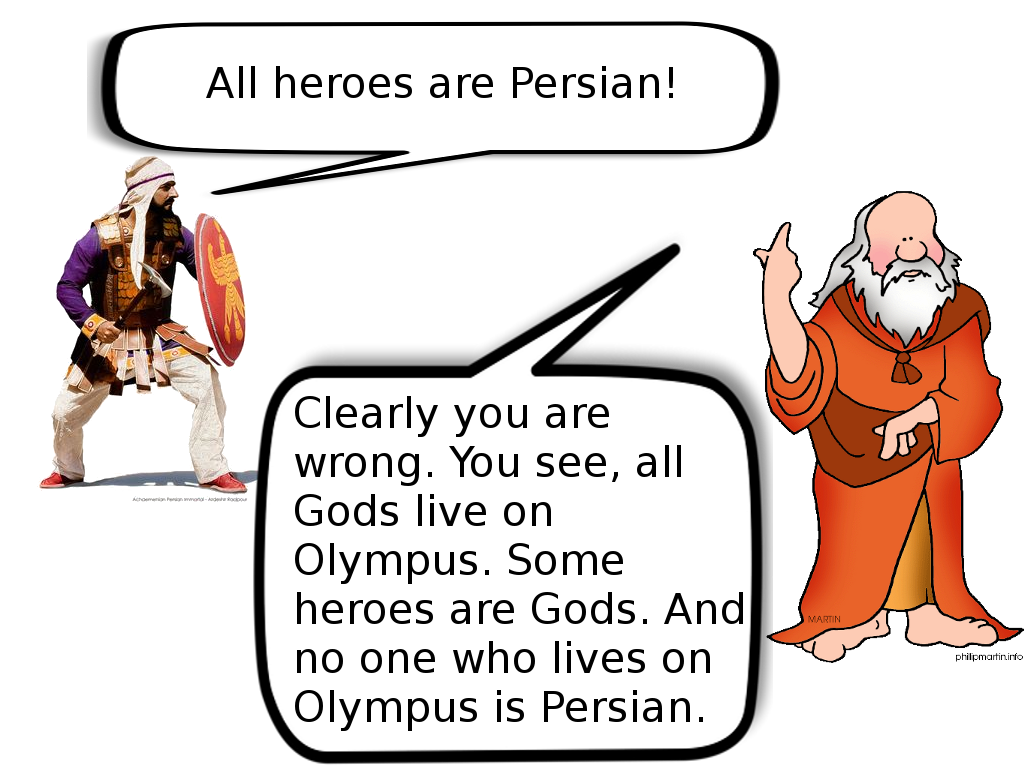
\includegraphics[height=7cm]{../img/persian_invaders.png}
\end{center}
\end{frame}

\begin{frame}[noframenumbering]{How Did You Solve This?}
\begin{center}
  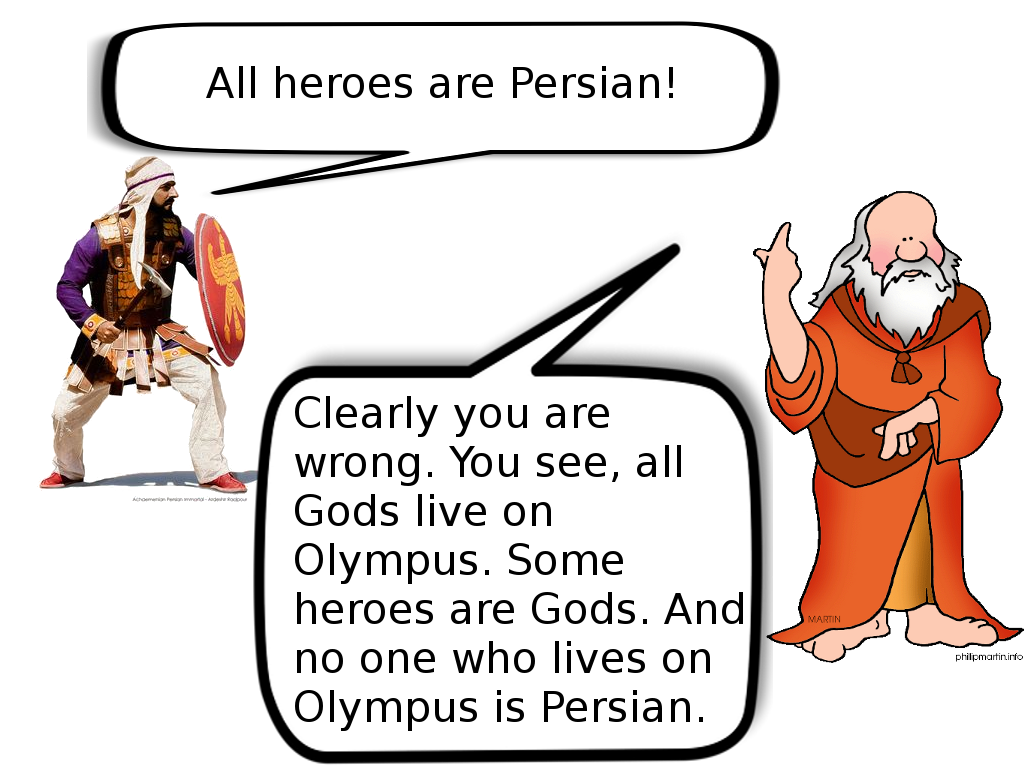
\includegraphics[height=7cm]{../img/persian_invaders.png}
\end{center}
\end{frame}

\begin{frame}[noframenumbering]{Show of Hands: First Order Logic?}
\begin{center}
\scalebox{0.5}{
$
\begin{nd}
\hypo {1} {\forall x~~\textrm{God}(x) \supset \textrm{LivesOnOlympus}(x)}
\hypo {2} {\exists x~~\textrm{Hero}(x) \land \textrm{God}(x)}
\hypo {3} {\lnot \exists x~~\textrm{LivesOnOlympus}(x) \land \textrm{Persian}(x)}

\open
  \hypo {4} {\forall x~~\textrm{Hero(x)} \supset \textrm{Persian}(x)}
  \open[a]
    \hypo {5}  {\textrm{Hero}(a) \land \textrm{God}(a)}                          \Ee{2}
    \have {6}  {\textrm{Hero}(a)}                                                \ae{5}
    \have {7}  {\textrm{Hero(a)} \supset \textrm{Persian}(a)}                    \Ae{4}
    \have {8}  {\textrm{Persian}(a)}                                             \ie{6,7}
    \have {9}  {\textrm{God}(a)}                                                 \ae{5}
    \have {10} {\textrm{God}(a) \supset \textrm{LivesOnOlympus}(a)}              \Ae{1}
    \have {11} {\textrm{LivesOnOlympus}(a)}                                      \ie{9,10}
    \have {12} {\textrm{LivesOnOlympus}(a) \land \textrm{Persian}(a)}            \ai{8,11} 
    \have {13} {\exists x~~\textrm{LivesOnOlympus}(x) \land \textrm{Persian}(x)} \Ei{12} 
  \close
  \have {14} {\exists x~~\textrm{LivesOnOlympus}(x) \land \textrm{Persian}(x)}   \r{12} 
  \have {15} {\bot}                                                              \by{$\bot$ I}{3,14}
\close
\have {16} {\lnot~~\forall x~~\textrm{Hero(x)} \supset \textrm{Persian}(x) }     \by{$\lnot$ I}{4--15}
\end{nd}
$
}
\end{center}
\end{frame}

%%%%%%%%%%%%%%%%%%% 
% SYLLOGISMS
%%%%%%%%%%%%%%%%%%%
\begin{frame}{Syllogisms: The First Natural Logic}
\begin{center}
\scalebox{0.5}{
  $
  \begin{nd}
  \hypo {1} {\ww{All Gods live on Mount Olympus}}
  \hypo {2} {\ww{Some heroes are Gods}}
  \hypo {3} {\ww{Nobody who lives on Mount Olympus is Persian}}
  \have {4} {\ww{Some heroes live on Mount Olympus}}  \by{AII (Darii)}{1,2}
  \have {5} {\ww{Some heroes are not Persian}}        \by{EIO (Ferio)}{4,3}
  \have {6} {\lnot~~\ww{All heroes are Persian}}      \by{SaP $\bot$ SoP}{5}
  \end{nd}
  $
}
\end{center}
\vspace{2ex}
\pause

\hh{...But syllogisms are cripplingly unexpressive}

\end{frame}

%%%%%%%%%%%%%%%%%%% 
% NATLOG ANIMATION
%%%%%%%%%%%%%%%%%%%
\input example.tex

%%%%%%%%%%%%%%%%%%%%%%%%%%%%%%%%%%%%%%%%%%%%%%%%%%%%%%%%%%%%%%%%%%%%%%%%%%%%%%%%
%% INFERENCE
%%%%%%%%%%%%%%%%%%%%%%%%%%%%%%%%%%%%%%%%%%%%%%%%%%%%%%%%%%%%%%%%%%%%%%%%%%%%%%%%
%
%
%%%%%%%%%%%%%%%%%%%% 
%% REMINDER
%%%%%%%%%%%%%%%%%%%%
%\begin{frame}[noframenumbering]{Problem Setup}
%\begin{center}
%  \teaserFullDerivation
%\end{center}
%\end{frame}

%%%%%%%%%%%%%%%%%% 
% EXAMPLE SEARCH
%%%%%%%%%%%%%%%%%%
\def\title{Natural Logic Inference as Search}
\def\no{\monoUpR{}{\textbf{No$_{\downarrow \downarrow}$}}{}{}}
\def\carnivores{\monoDownR{felines}{carnivores}{animal}{organism}}
\def\eat{\monoDownR{slurp}{eat}{consume}{}}
\def\animals{\monoDownR{chordate}{animals}{organism}{living thing}}
\begin{frame}{\title}
  \begin{center}
    \hh{Shorthand for a node:} \\
    \vspace{0.5cm}
    \scalebox{0.75}{\no \carnivores \eat \animals} \\
    \vspace{0.5cm}
    
\includegraphics[height=2.0cm]{../img/dArrow.jpg} \\
    \vspace{0,5cm}
      \setstyles
      \begin{tikzpicture}[grow=down, sloped]
      \node[boxfact](main) {\w{No carnivores eat animals?}};
      \end{tikzpicture}
  \end{center}
\end{frame}

\input exampleSearch2pane.tex



%%%%%%%%%%%%%%%%%% 
% CONTRIBUTIONS
%%%%%%%%%%%%%%%%%%
\begin{frame}{Three Contributions for Generalizable Inference}
\begin{enumerate}
\item \hh{Partial order over meronymy + relations}
  \begin{center}
  \begin{tabular}{ccc}
    \monoUp{Berlin}{Germany}{EU}{Earth} &
    &
    \monoUp{sell}{own}{have}{}
  \end{tabular}
  \end{center}
\pause

\item \hh{Natural Logic over dependency trees}

\begin{center}
\begin{dependency}[text only label, label style={above}]
  \begin{deptext}[column sep=-0.00cm]
    \tagUp{Some} \& \tagUp{truly} \& \tagUp{\darkred{notorious}} \& 
      \tagUp{villains} \& \tagUp{have} \& \tagUp{lairs} \&[-1ex] .\\
  \end{deptext}
  \depedge[edge unit distance=1.0ex]{5}{1}{operator}
  \depedge[edge unit distance=1.25ex]{5}{4}{nsubj}
  \depedge[edge unit distance=1.25ex, edge style={darkred!100!black,thick}]{4}{3}{\darkred{amod}}
  \depedge[edge unit distance=1.25ex, edge style={darkred!100!black,thick}]{3}{2}{advmod}
  \depedge[edge unit distance=1.25ex]{5}{6}{dobj}
\end{dependency}
\end{center}
\pause

\item \hh{Hybrid statistical / logical solver}

\end{enumerate}
\end{frame}
